% Lazy Coulomb Planner: draft paper.
%
% Upload the whole `paper/` folder to Overleaf (main.tex, refs.bib, figures/*.pdf).
% Compiler: pdfLaTeX. Class: IEEEtran (built into Overleaf).
%
% Numbers in this draft come from the experiments in ../experiments/, planner
% version v2.1.0 (optimised build), unless a sentence says otherwise. Text in red,
% written with \pending{...}, is waiting for results that are still running or for
% a decision by the authors. refs.bib was checked against the publishers' records
% on 18 Nov 2026 (refs_check.md); recheck R2+ for a journal version before submission.

\documentclass[conference]{IEEEtran}

\usepackage[utf8]{inputenc}
\usepackage[T1]{fontenc}
\usepackage{amsmath,amssymb}
\usepackage{graphicx}
\usepackage{booktabs}
\usepackage{xcolor}
\usepackage{tikz}
\usetikzlibrary{arrows.meta,calc,decorations.pathmorphing}
\usepackage{algorithm}
\usepackage{algpseudocode}
\usepackage{siunitx}
\sisetup{group-minimum-digits=4}
\usepackage{cite}
\usepackage[hidelinks]{hyperref}

\newcommand{\pending}[1]{\textcolor{red}{[#1]}}
\newcommand{\lcp}{LCP}

\begin{document}

\title{Lazy Coulomb Planner: Checking and Repairing\\the Straight Line Before Searching the Grid}

\author{
\IEEEauthorblockN{Kaveesha Dhananjaya}
\IEEEauthorblockA{Senior Robotics Engineer, Hype Insight Global\\New South Wales, Australia\\kaveeshadhananjaya2002@gmail.com}
% Single author. The supervisor will proof-read at the end (acknowledgement).
}

\maketitle

\begin{abstract}
Grid-based global planners spend most of their time searching free space, even
when the straight line from start to goal is almost clear. The Lazy Coulomb Planner
(\lcp), a global planner for the ROS~2 Navigation stack (Nav2), checks the straight
line on the costmap first; most of its speed comes from this check together with a
weighted A\textsuperscript{*} when the line is blocked. Before that search, a lazy
correction pushes each blocked point sideways within a small attempt budget,
choosing the side with a Coulomb-like repulsion or a cheaper probe; both beat a
fixed side. The correction makes the planner a further 1.3 to 2.7 times faster on
sparse and large maps and up to 2.6 times slower at 20\,\% obstacle density and above.
On 69 generated maps \lcp{} solved all \num{6234} routable pairs without entering
the inscribed zone and refused all 666 pairs without a route. On \SI{50}{m} maps it
is 66 times faster than the fastest Nav2 grid planner at 2.5\,\% density and 2.6
times at 40\,\%; against NavFn switched to A\textsuperscript{*}, the fastest tuned
grid planner, it is 11 times faster at 10\,\% and as fast at 40\,\%. Jump point
search, Anya and R2, which Nav2 does not provide, are faster still. In simulated
driving \lcp{} reached a similar number of goals to NavFn, with more recovery
behaviours under Regulated Pure Pursuit and a similar number under MPPI.
\end{abstract}

\begin{IEEEkeywords}
path planning, mobile robots, Nav2, ROS 2, lazy planning
\end{IEEEkeywords}

% ---------------------------------------------------------------------------
\section{Introduction}

The global planner of a mobile robot is called whenever a goal is set and, in
Nav2's default behaviour tree, again once a second while the robot drives. The
planners shipped with Nav2~\cite{macenski2020marathon}, the standard navigation
system of ROS~2, are grid searches: NavFn (a wavefront Dijkstra or
A\textsuperscript{*} on the costmap), Smac~2D~\cite{macenski2024smac} and
Theta\textsuperscript{*}~\cite{daniel2010theta}, in its Lazy Theta\textsuperscript{*}
variant~\cite{nash2010lazy}. Their cost grows with the area they
have to explore, which is large when the map is large, even if the robot could
almost drive straight to the goal.

Many environments are mostly open: warehouses with aisles, halls, outdoor areas,
the space a drone or a ground robot explores between frontiers. For these we ask
a different question: instead of searching for a path, how little work is needed
to repair the obvious one? This paper answers it with a planner that

\begin{itemize}
\item starts from the straight line and checks it against the costmap;
\item where it is blocked, inserts a waypoint and pushes it sideways until it is
  clear, choosing the side with a repulsion summed over nearby obstacle cells, in
  the spirit of Coulomb's law, or with a cheaper probe of both sides;
\item locks the cleared waypoint and continues along the path, backing up to try
  the other side when a choice leads nowhere;
\item hands the request to a weighted A\textsuperscript{*} search on the same
  costmap when the correction exceeds a small budget, so that a path is returned
  whenever one exists; and
\item never returns a path that enters the inscribed zone, where the robot's
  body would touch an obstacle.
\end{itemize}

Our measurements show that most of the speed-up over Nav2's planners does not
come from the correction. Checking the straight line and running a weighted
A\textsuperscript{*} when it is blocked already gives the larger part. The correction
adds to it on sparse and large maps and costs time on dense ones.

The contributions are: (i) the planner and its open-source Nav2 implementation;
(ii) a controlled benchmark that varies obstacle density, map size, obstacle
shape and corridor width one at a time, with ground-truth routability, against
the three Nav2 grid planners at their defaults and with their cost terms switched
off; (iii) ablations of the main design choices, including a comparison with the
heuristic of checking the straight line and otherwise running
A\textsuperscript{*}, and with jump point search, Anya and R2 outside Nav2; and (iv)
simulated driving experiments with two path-following controllers, including one
with \lcp{}'s path reuse switched off.

% ---------------------------------------------------------------------------
\section{Related work}
\label{sec:related}

\emph{Grid and sampling planners.} Dijkstra's algorithm~\cite{dijkstra1959note}
and A\textsuperscript{*}~\cite{hart1968formal} pay for every cell they expand,
so their cost grows with path length on open maps and towards the map's area in
clutter; weighted A\textsuperscript{*}~\cite{pohl1970heuristic}, which our
fallback uses, trades optimality for fewer expansions. Jump point
search~\cite{harabor2011jps}, extended to 3D in~\cite{liu2017sfc}, prunes
symmetric grid paths without preprocessing but still expands outwards from the
start. Sampling-based planners such as RRT-Connect~\cite{kuffner2000rrt} pay per
sample instead. Nav2 ships NavFn, Smac~2D and
Theta\textsuperscript{*}~\cite{macenski2020marathon,macenski2023survey,macenski2024smac};
its maintainers report tens of milliseconds per plan on $100\times100$\,m maps
and, for Smac~2D, more than a second on a large warehouse map~\cite{macenski2024smac}.

\emph{Any-angle and vector-based planners.}
Theta\textsuperscript{*}~\cite{daniel2010theta} adds line-of-sight checks to a
full A\textsuperscript{*} expansion, and Anya~\cite{harabor2016anya} finds
optimal any-angle paths by searching over intervals; see~\cite{nash2013anyangle}
for a survey and~\cite{uras2015comparison} for a comparison. Closest to our
cost argument are the vector-based planners: RayScan~\cite{hechenberger2020rayscan}
and R2~\cite{lai2024r2} with its successor R2+~\cite{lai2024r2plus} cast a ray
towards the goal and go around only what the ray hits, so their work, like ours,
depends on the obstacles met rather than on the free area, and they return optimal
paths. We do not claim this property as new.
RayScan works on polygons and R2 and R2+ on binary occupancy grids; \lcp{} differs
in working directly on an inflated Nav2 costmap, which it thresholds at the
inscribed cost and whose costs it uses for the margin and the post-processing,
in committing to one side per
obstacle greedily instead of exploring both, and in bounding its worst case with
a grid search; it gives up optimality in return.
The authors of R2 publish a C++ implementation on binary grids~\cite{r2code}, which
we run on our maps alongside Anya and jump point search (Section~\ref{sec:outside});
for R2+ and RayScan we found none.

\emph{Straight-line-first repair.} Starting from the straight line and inserting
intermediate goals where it is blocked is an old idea: Lozano-P{\'e}rez and
Wesley~\cite{lozanoperez1979algorithm} describe Udupa's recursive
scheme~\cite{udupa1977collision} of this kind and criticise it for using only local information. RMPD~\cite{li2018rmpd}
recursively displaces the midpoint of a blocked segment at random and does not
backtrack, and APPATT~\cite{liu2022appatt} chooses between tangent points by
rules. Bug algorithms~\cite{lumelsky1987path,kamon1998tangentbug} follow obstacle
boundaries with local sensing, and FAR Planner~\cite{yang2022far} maintains a
visibility graph. \lcp{} shares the recursive skeleton; its contributions are
the deterministic perpendicular push with a margin on the costmap, the
repulsion-based side choice, bounded backtracking over sides, and the grid
fallback, which makes it resolution-complete on the costmap. The simplest member of this
family, ``check the straight line, otherwise run A\textsuperscript{*}'', is a
widely used heuristic for which we found no primary source; Section~\ref{sec:outside}
measures how much of \lcp{}'s speed it already explains.

\emph{Lazy search.} Lazy planners assume edges are free and check them only on
the candidate path, repairing it when a check fails~\cite{bohlin2000lazy,mandalika2019gls}.
That literature saves collision checks that are expensive; on a costmap a check
is cheap, and \lcp{}'s laziness is about search work instead: it does not
expand free space that the straight line already crosses.

\emph{Potential fields and Coulomb planners.} Artificial potential
fields~\cite{khatib1985real} steer down the gradient of an attractive goal and
repulsive obstacles and suffer from local minima~\cite{koren1991potential};
later work changed the potential functions~\cite{ge2000new}, made them free of
local minima~\cite{rimon1992exact}, or modelled obstacles as electrostatic
charges~\cite{valavanis2000electrostatic}. Coulomb's law has recently been used
to shape the neighbour sets of sampling-based planners~\cite{zhang2024fdit}.
We are not the first to use a Coulomb-like repulsion in planning. In \lcp{}
the repulsion is not followed as a gradient: only its sign is used, to choose on
which side a blocked waypoint leaves its obstacle, and a wrong choice is undone
by backtracking or the fallback.

\emph{Deformation, smoothing and clearance.} Elastic
bands~\cite{quinlan1993elastic} and the timed elastic band~\cite{rosmann2012teb,rosmann2017teb}
deform a collision-free initial path; CHOMP~\cite{ratliff2009chomp},
TrajOpt~\cite{schulman2014trajopt} and EGO-Planner~\cite{zhou2021ego} can start
from a straight line that runs through obstacles and push it out by continuous
optimisation. EGO-Planner is the closest modern analogue to \lcp{}: it also
pushes colliding segments away with a safety distance, but by gradient
descent, where \lcp{} makes one discrete push per obstacle, and it chooses the
direction of the push from a collision-free guiding path found by
A\textsuperscript{*} for each colliding segment, where \lcp{} uses the sign of a
local repulsion. Shortcutting a path
trades clearance for length~\cite{geraerts2007creating}, and paths of minimal
length lie at the zero-clearance end of the spectrum between visibility graphs and
Voronoi diagrams~\cite{wein2008planning}. \lcp{}'s paths are of this short kind
and keep less clearance than NavFn's, which pays a cost for every cell near an
obstacle; Section~\ref{sec:ablations} shows that in \lcp{} the clearance is lost
by the correction itself, before any shortcutting. The distance map planner of
the jps3d library~\cite{jps3d} also adds clearance after a grid search: it
builds a potential field around the obstacles and searches again for a safer
path in a region around the jump point search path. \lcp{}'s clearance step
(Section~\ref{sec:post}) instead pushes the existing waypoints locally.

% ---------------------------------------------------------------------------
\section{Method}
\label{sec:method}

\subsection{Problem}

Given a 2D costmap $C$, in which a cell is treated as an obstacle if its cost is at
least $c_\text{insc}$ (253, Nav2's \texttt{INSCRIBED\_INFLATED\_OBSTACLE}; lethal
cells have 254), and a start $s$ and goal $g$ in free cells, find a polyline from
$s$ to $g$ whose segments touch no obstacle cell, or report that none exists.
Cells with lower inflation costs are free; \lcp{} may cross them and uses their
cost only to limit the margin push (Section~\ref{sec:lazy}) and in post-processing. Segments are checked
with an exact grid traversal~\cite{amanatides1987fast} that visits every cell a
segment touches, extended so that a segment through the corner shared by four
cells counts as touching all of them.

\subsection{Lazy correction}
\label{sec:lazy}

The path starts as $[s, g]$. Segments are scanned in order; the first segment
that touches an obstacle gets a new waypoint $w$ in the first obstacle cell it
enters (Fig.~\ref{fig:idea}). The waypoint $w$ is pushed along the unit normal
$\mathbf{n}$ of that segment until it reaches free space, and then a further
margin $\mu$ (\SI{0.5}{m}) as long as the way is free and the cost does not rise,
which leaves room to round the corner later. The pushed waypoint is locked, and
scanning resumes with the new segment that ends at it. The branch fails if $w$ is
not free after 400 push steps, if it ends within half a cell of either end of the
segment it was inserted into (the same correction would then repeat), or if the
path becomes longer than five times the straight-line distance plus 20 cells.

\begin{figure*}[t]
\centering
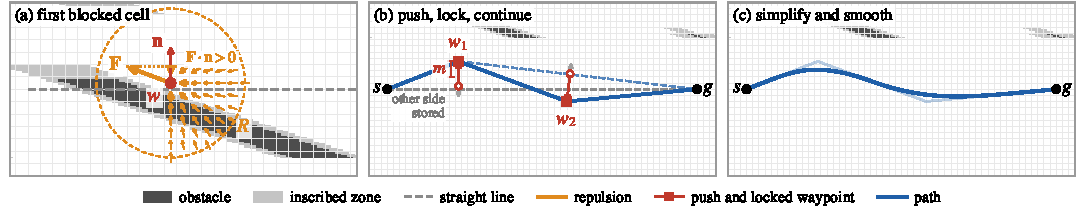
\includegraphics[width=\textwidth]{figures/method_idea.pdf}
\caption{Lazy correction on a costmap; cells in the inscribed zone count as
obstacles. (a) The straight line from $s$ to $g$ is blocked; a waypoint $w$ is
placed in the first blocked cell. Every blocked cell within $R$ repels $w$ (small
arrows, thicker where stronger); the side is the sign of the summed
repulsion $\mathbf{F}$ along the segment normal $\mathbf{n}$. Here $\mathbf{F}$
points mostly backwards, but the mass of the obstacle below the line gives it an
upward component, so $w$ leaves over the top. (b) $w$ is pushed along $\mathbf{n}$
until it is free and then by a further margin $\mu$, and locked as $w_1$; the other
side is stored for backtracking. The next blocked segment (dashed) is corrected
the same way, and here the repulsion of the second obstacle sends $w_2$ the other
way. Free space and the obstacles off the line cost no work. (c) Simplification and
corner smoothing give the final path (the lazy path is shown faint). The geometry
is computed with the method's rules on a toy grid.}
\label{fig:idea}
\end{figure*}

\subsection{Choosing the side with a Coulomb-like repulsion}

The key decision is on which side $w$ leaves the obstacle. Every obstacle cell
$c$ within a charge radius $R$ (\SI{1}{m}) of $w$ contributes
\begin{equation}
\mathbf{F}(w) = \sum_{c:\,\|w-c\|\le R} \frac{w - c}{\max(\|w - c\|,\tfrac12)^{\,p+1}},
\qquad p = 2,
\end{equation}
a repulsion of magnitude $1/\|w-c\|^{p}$ pointing away from $c$, with distances in
cells and softened below half a cell. The sign of $\mathbf{F}\cdot\mathbf{n}$
selects the side, where $\mathbf{n}$ is the left normal of the segment; if
$|\mathbf{F}\cdot\mathbf{n}| < 0.05$ the force counts as balanced and $w$ goes
left. While $\mathbf{F}\cdot\mathbf{n}$ points to the chosen side, its magnitude
sets the step length, clamped between a quarter of a cell and one cell; otherwise
the step is one cell, so the push cannot stall where the force vanishes. The side
chosen on the first step is kept for the whole push: letting the force reverse
the waypoint at every step makes it oscillate between obstacles
(Section~\ref{sec:ablations}). The exponent matters little; $p = 1$ performs the
same (Section~\ref{sec:ablations}).

The side rule is a parameter of \lcp{}. Besides the Coulomb rule, which is the
default, it offers a cheaper \emph{probe} rule: step from $w$ along $+\mathbf{n}$
and $-\mathbf{n}$ and take the side that reaches free space in fewer steps (left on a tie). The
rest of the method is the same for both. Section~\ref{sec:ablations} compares
them with each other and with a fixed side.

\subsection{Backtracking to the other side}

Every placed waypoint could have left its obstacle on the other side. That
alternative is stored together with the path as it was. When a branch fails, the
search resumes from the stored alternative with the shortest partial path. The
total number of placement attempts, retries included, is limited to a budget $B$
(50).

\subsection{Fallback and early refusal}

After 25 attempts (half the default budget; this count is fixed and does not
change with $B$) a breadth-first search grown from both the start and the goal,
capped at \num{20000} cells, checks whether either is sealed inside a small
pocket; if so, the request is refused at once. With a budget below 25 this check
never runs. When the budget is used up, a weighted A\textsuperscript{*} search
(heuristic weight 3, each cell expanded once) over the free cells of the same
costmap finds a route or proves there is none. Both searches are 8-connected and
never move diagonally between two obstacle cells that touch at a corner. The
route is then treated like a lazy path. This makes \lcp{} resolution-complete on
the costmap; Section~\ref{sec:results} reports how much of the work the fallback
does.

\subsection{Post-processing}
\label{sec:post}

The waypoints are simplified by joining each to the farthest later waypoint it can
reach in a straight line; this removes the back-and-forth tangles the lazy search
can leave around a single obstacle. A clearance step then moves waypoints and
inserts new ones along the repulsion while the costmap cost keeps falling, until
a comfort cost of 30 is reached, by at most \SI{1}{m} (an inserted point also by
less than 0.35 of its distance to the neighbouring waypoints), keeping every
change collision-free. Corners are rounded
with Chaikin's corner cutting~\cite{chaikin1974algorithm}, five passes, where each
cut is kept only if the new chord is clear; this makes the smoothed path
collision-free by construction. Finally the path is resampled to poses
\SI{0.1}{m} apart, keeping original vertices where a chord would touch an
obstacle, and checked once more as a whole.

\subsection{Driving}
\label{sec:drivemethod}

Nav2 replans about once a second. A fresh plan from a start that has moved a few
centimetres can choose the other side of an obstacle; a path that jumps like that
steers the follower towards the obstacle. When a request has the same goal as the
previous one and the robot is within \SI{0.5}{m} of the previous path, \lcp{}
keeps that path while it is still collision-free, and switches to a fresh plan
only if it is at least 15\,\% shorter. A start or goal that lies on an occupied
cell is moved to the nearest free cell within \SI{0.5}{m}. Path reuse is off in
every planner benchmark (each request is planned from scratch) and on in the
driving tests, where Section~\ref{sec:driving} also measures \lcp{} without it.

\begin{algorithm}[t]
\caption{Lazy correction with backtracking}
\label{alg:lcp}
\begin{algorithmic}[1]
\State $P \gets [s, g]$; $i \gets 0$; $A \gets \emptyset$; $k \gets 0$
\While{$i < |P| - 1$}
  \If{segment $(P_i, P_{i+1})$ is clear} $i \gets i + 1$; \textbf{continue}
  \EndIf
  \State $w \gets$ first obstacle point on $(P_i, P_{i+1})$
  \State $\sigma \gets \operatorname{sign}(\mathbf{F}(w)\cdot\mathbf{n})$
  \State store $(P, i, w, -\sigma)$ in $A$
  \Repeat
    \State $k \gets k + 1$; \textbf{if} $k > B$ \textbf{then return} fallback$(s, g)$
    \If{$k = 25$ \textbf{and} $s$ or $g$ is sealed in a pocket}
    \Statex \hspace{\algorithmicindent}\hspace{\algorithmicindent}(BFS from both, \num{20000} cells)
      \State \Return no path
    \EndIf
    \State try to push $w$ on side $\sigma$ and insert it after $P_i$
    \Statex \hspace{\algorithmicindent}\hspace{\algorithmicindent}(fails if not cleared, near $P_i$ or $P_{i+1}$, or too long)
    \If{failed}
      \If{$A = \emptyset$} \Return fallback$(s, g)$ \EndIf
      \State remove the entry of $A$ with the shortest path
      \Statex \hspace{\algorithmicindent}\hspace{\algorithmicindent}\hspace{\algorithmicindent}and set $(P, i, w, \sigma)$ to it
    \EndIf
  \Until{inserted}
\EndWhile
\State \Return post-process$(P)$
\end{algorithmic}
\end{algorithm}

\subsection{Implementation}

\lcp{} is a C++ plugin for the Nav2 planner server on ROS~2 Jazzy, about
\num{1700} lines, with 18 unit tests. It is open source at
\url{https://github.com/KD-27/Lazy-Coulomb-Planner/tree/paper-v2}, together with
the benchmark, the simulation tooling and the raw results of every experiment
in this paper. All parameters have defaults; the values above are those
defaults.

% ---------------------------------------------------------------------------
\section{Experimental setup}
\label{sec:setup}

\subsection{Planner benchmark}
\label{sec:bench}

Maps are generated at a resolution of \SI{5}{cm} with a fixed seed: square maps
with random circular obstacles of radius \SIrange{0.3}{0.8}{m} placed until a
target fraction of cells is occupied (0 to 45\,\%; at higher densities the free
space falls apart), maps from \SI{10}{m} to \SI{200}{m} at 10\,\%, maps with
square or concave U-shaped obstacles, and regular grids of \SI{4}{m} blocks with
corridors of 0.8, 1.2, 2 and \SI{3}{m}. These 21 maps form the \emph{controlled
suite}. To put error bars on the main trends, the maps are generated again with
other seeds: the ten non-empty densities with four more seeds each (40 maps), the
\SI{10}{m}, \SI{25}{m} and \SI{100}{m} maps with two more (6), and the U-shaped
map with two more (2). Every non-empty \SI{50}{m} density map, including the one at 10\,\%, thus has
five seeds, the other sizes and the U-shaped map three, and the empty and \SI{200}{m} maps
one: 69 maps in all. The costmap is Nav2's static layer plus inflation (robot
radius \SI{0.22}{m}, inflation radius \SI{0.7}{m}).

For every map, 100 start--goal pairs at least \SI{3}{m} apart are drawn with a
fixed seed from cells with cost below 210. Every pair is planned five times by
every planner through Nav2's planner server; the time used is the median of the
five as reported by the server. \lcp{}'s path reuse is off, so all five are
planned from scratch. NavFn, Smac~2D and Theta\textsuperscript{*} run with their
Nav2 defaults and, in a separate run on the controlled suite
(Section~\ref{sec:tuned}), with their cost terms switched off. All three are the
release builds of the Nav2 Jazzy binary packages.

Whether a pair has a route is decided from the map alone, not by any planner:
cells within the inscribed radius of an obstacle are blocked, and a pair is
routable if start and goal lie in the same 4-connected free region (which is
the connectivity of \lcp{}'s 8-connected searches without corner cutting). A
returned path counts as solved only if it touches no cell with cost 253 or more,
that is, no cell on which the robot's body would be in contact with an obstacle.

\subsection{Ablations}

Each design choice is varied alone, the others at their defaults, on eight maps:
\SI{50}{m} maps at 10, 20 and 30\,\% density, with U-shaped obstacles and with
\SI{1.2}{m} corridors, and three indoor maps at \SI{5}{cm} resolution (a maze of
$20\times25$\,m, a house of $19\times11$\,m and an event venue of $20\times20$\,m,
drawn by the author as typical indoor layouts, with no particular source), 100 pairs each, every pair planned three
times.

\subsection{Driving}

A simulated TurtleBot3 Waffle~\cite{turtlebot3} drives a fixed sequence of 15
goals in Nav2's sandbox world in Gazebo~\cite{koenig2004gazebo}, with the full
Nav2 stack (AMCL~\cite{dellaert1999mcl,fox2003kld}, behaviour tree, recovery behaviours) and
either Regulated Pure Pursuit~\cite{macenski2023rpp} or
MPPI~\cite{williams2017mppi} as the path follower; only the global planner
changes between runs. Goals are drawn with a fixed seed from
cells at least \SI{0.3}{m} from obstacles. Runs are made one at a time on an
otherwise idle machine; 10 runs per planner with each follower (with MPPI, five
on each of two days, the four planners interleaved).

The same robot also drives 10 goals in six worlds built from generated maps
(\SI{20}{m} square: open, 10, 20 and 30\,\% obstacle density, U-shaped
obstacles, and \SI{1.2}{m} corridors), whose obstacles match the map cells
exactly, three runs per planner with Regulated Pure Pursuit. Here the robot's
pose is the simulator's wheel odometry: with AMCL, the robot was mislocalised
among the many identical cylinders, which is not what the test is meant to
measure.

All experiments ran on one laptop (Intel Core i7-13620H, \SI{16}{GB} RAM, Ubuntu
24.04, ROS~2 Jazzy, Nav2 1.3.13), with \lcp{} compiled with optimisation.

% ---------------------------------------------------------------------------
\section{Results}
\label{sec:results}

\subsection{Planning time against obstacle density}

\begin{figure}[t]
\centering
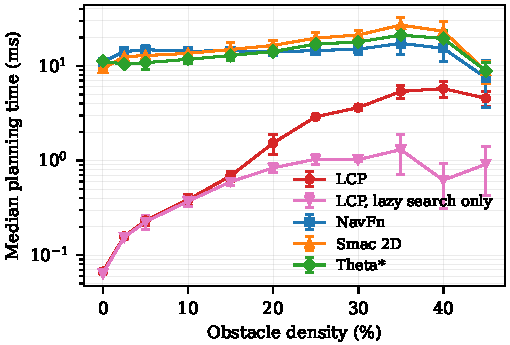
\includegraphics[width=\columnwidth]{figures/time_vs_density.pdf}
\caption{Median planning time on \SI{50}{m} maps against obstacle density, mean and
standard deviation over five seeds (one map at 0\,\%). The lazy-search-only curve
covers only the requests it solves itself.}
\label{fig:time_density}
\end{figure}

\begin{table}[t]
\centering
\caption{\lcp{} against the fastest grid planner on \SI{50}{m} maps. Median
planning time: mean $\pm$ standard deviation over five seeds. Tail (95th
percentile / slowest plan): solved requests of all five seeds pooled; NavFn has
the lowest tail of the three grid planners at every density.}
\label{tab:density}
\setlength{\tabcolsep}{2.5pt}
\footnotesize
\begin{tabular}{@{}rccccc c@{}}
\toprule
 & \multicolumn{3}{c}{Median (ms)} & & \multicolumn{2}{c}{p95 / max (ms)} \\
\cmidrule(lr){2-4}\cmidrule(l){6-7}
Density & \lcp{} & Fastest grid & Speed-up & Lazy only & \lcp{} & NavFn \\
\midrule
2.5\,\% & $0.16 \pm 0.01$ & $10.4 \pm 0.4$ & $66 \pm 4$ & 99\,\% & 0.43 / 3.7 & 24 / 27 \\
10\,\%  & $0.39 \pm 0.05$ & $11.8 \pm 1.2$ & $31 \pm 3$ & 96\,\% & 2.2 / 4.0  & 25 / 28 \\
20\,\%  & $1.53 \pm 0.36$ & $13.5 \pm 0.9$ & $9 \pm 2$  & 71\,\% & 4.5 / 8.1  & 24 / 26 \\
30\,\%  & $3.63 \pm 0.25$ & $15.0 \pm 1.9$ & $4.1 \pm 0.5$ & 37\,\% & 6.7 / 10 & 27 / 31 \\
40\,\%  & $5.76 \pm 1.16$ & $14.9 \pm 4.0$ & $2.6 \pm 0.4$ & 17\,\% & 20 / 28  & 42 / 95 \\
45\,\%  & $4.55 \pm 0.85$ & $6.5 \pm 2.4$  & $1.5 \pm 0.4$ & 29\,\% & 9.2 / 13 & 25 / 45 \\
\bottomrule
\end{tabular}
\end{table}

Fig.~\ref{fig:time_density} and Table~\ref{tab:density} show the central result.
The grid planners' times change little with density: the fastest of them takes 10
to \SI{15}{ms} from 2.5 to 40\,\% (Smac~2D's median exceeds \SI{20}{ms} at 35\,\%,
Fig.~\ref{fig:time_density}), because their cost is set by the area they explore;
at 45\,\% they are faster, \SI{6.5}{ms}, because the few routable pairs lie in small
connected regions. \lcp{} takes \SI{0.16}{ms} at 2.5\,\% density, 66 times less,
and its time rises with density as more corrections are needed and more requests
go to the fallback. It remains faster than the fastest grid planner up to 45\,\%,
the densest maps on which random start--goal pairs are still mostly connected; at
45\,\% only 9 to 40 of the 100 pairs per map have a route, so that row rests on
few requests. The ``lazy only'' column shows the share of requests the lazy
correction solves without the fallback: almost all at low density, about a third
at 30\,\%. The fallback gives \lcp{} a heavier tail than its median suggests, but
its 95th percentile stays below NavFn's on every density, and below NavFn's
\emph{median} up to 30\,\%.

\subsection{Planning time against map size}

\begin{figure}[t]
\centering
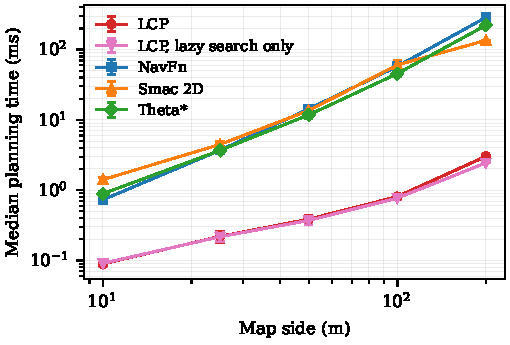
\includegraphics[width=\columnwidth]{figures/time_vs_size.pdf}
\caption{Median planning time against the side of a square map at 10\,\% obstacle
density (five seeds at \SI{50}{m}, three at the other sizes, one at \SI{200}{m}).}
\label{fig:time_size}
\end{figure}

The advantage grows with the size of the map (Fig.~\ref{fig:time_size}):
$8.0 \pm 0.4$ times at \SI{10}{m}, $16 \pm 3$ at \SI{25}{m}, $31 \pm 3$ at
\SI{50}{m} and $56 \pm 2$ at \SI{100}{m}. On the single \SI{200}{m} map \lcp{}
plans in \SI{3.0}{ms} against \SI{286}{ms} for NavFn and \SI{221}{ms} for
Theta\textsuperscript{*} (\SI{3.3}{ms} and \SI{304}{ms} for \lcp{} and NavFn in
the separate run of Table~\ref{tab:outside}, which repeats the controlled suite;
the two runs differ by up to 10\,\% on this map). Smac~2D fails 42 of the 100
requests there by reaching its default iteration limit, so its point in
Fig.~\ref{fig:time_size} covers only the 58 it solves. \lcp{}'s time grows roughly with the length of the
path, the grid planners' with the area of the map.

\subsection{Reliability}

\begin{figure}[t]
\centering
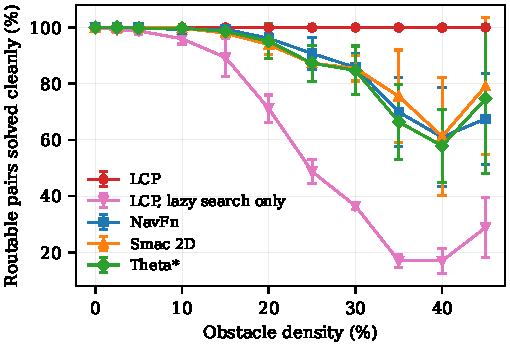
\includegraphics[width=\columnwidth]{figures/clean_vs_density.pdf}
\caption{Share of routable pairs solved with a path that does not enter the inscribed
zone, against obstacle density, \SI{50}{m} maps, five seeds.}
\label{fig:clean}
\end{figure}

Over all 69 maps \lcp{} solved every one of the \num{6234} routable pairs with a clean
path and refused every one of the 666 pairs without a route.

The grid planners return more paths that touch the inscribed zone as the density
grows (Fig.~\ref{fig:clean}): over all maps NavFn 439, Smac~2D 499 and
Theta\textsuperscript{*} 492, and at 40\,\% density only about 60\,\% of their
paths are clean. This is mainly an effect of their default configuration rather
than of the algorithms. At their Nav2 defaults they plan on the costmap's costs
and treat inscribed cells as very expensive but traversable, so on dense maps the
cheapest path sometimes grazes an obstacle; \lcp{} treats the same cells as walls.
We therefore do not count this
against the grid planners' search, and report it to show what each planner
returns out of the box on the same costmap. One case is not a matter of
configuration: Smac~2D returned 49 paths for pairs without a route, slipping
diagonally between two blocked cells that touch at a corner, which the robot
cannot pass.

\subsection{Obstacle shape and corridors}

With concave U-shaped obstacles (three seeds) \lcp{} plans in
$2.5 \pm 0.6$\,ms against $13.6 \pm 0.5$\,ms for NavFn, the fastest grid planner
there, although the lazy search alone solves only $45 \pm 11$\,\% of the pairs. Between \SI{4}{m} blocks it is 2.7 times faster than the fastest
grid planner with \SI{0.8}{m} corridors and 27 times with \SI{3}{m} corridors.

\subsection{Worst case and path quality}
\label{sec:quality}

Over all 69 maps, \lcp{}'s 95th-percentile planning time is \SI{6.9}{ms} and its
slowest plan \SI{28}{ms}, against 95th percentiles of 48 to \SI{77}{ms} and
slowest plans of 0.4 to \SI{0.8}{s} for the grid planners (on the \SI{200}{m}
map). Refusing a request without a route took \lcp{} at most \SI{63}{ms}.
\lcp{} paths are 1 to 3\,\% shorter than
NavFn's and turn far less (4.4 against 20.7 radians of total heading change on the
ablation maps), but they run closer to obstacles: the average costmap cost along
the path is about 16 on the \SI{50}{m} map at 10\,\% density against 0.4 for
NavFn, which follows the cost gradient into the middle of free space. 2.3\,\% of
\lcp{} paths keep a corner sharper than \SI{90}{\degree}.

Requests that need the fallback are harder, not worse served. Over the 69 maps
the lazy correction solved \num{4471} requests and the fallback \num{1763}. The fallback's
paths are as short relative to NavFn's as the lazy ones (median length ratio 0.96
against 0.98) and their higher costmap cost (79 against 21) mirrors NavFn's on the
same pairs (26 against 1.2): they are the pairs that run through clutter.

\subsection{Ablations}
\label{sec:ablations}

\begin{table}[t]
\centering
\caption{Ablations on eight maps (704 routable pairs). ``Lazy only'': solved
without the fallback. Time: mean over maps of the median planning time, with the
fallback on. Each block is a separate run with its own default row; the default
varies by about 3\,\% between runs, so smaller differences are noise. The first
block's rows were measured together in one run.}
\label{tab:ablation}
\setlength{\tabcolsep}{3pt}
\begin{tabular}{@{}llcc@{}}
\toprule
Choice & Variant & Lazy only & Time (ms) \\
\midrule
Side rule   & Coulomb $1/d^2$ (default)   & 489 & 1.21 \\
            & nearest free side (probe)   & 449 & 0.81 \\
            & fixed side (left first)     & 440 & 1.70 \\
\midrule
Force law   & $1/d^2$, side kept (default) & 489 & 1.23 \\
            & $1/d$, side kept            & 489 & 1.16 \\
            & $1/d^2$, may reverse        & 443 & 2.77 \\
\midrule
Margin $\mu$ & \SI{0}{m}                   & 305 & 1.58 \\
            & \SI{0.5}{m} (default)       & 489 & 1.24 \\
            & \SI{1.0}{m}                 & 509 & 1.16 \\
\midrule
Budget $B$  & 10                          & 249 & 1.25 \\
            & 25                          & 405 & 1.14 \\
            & 50 (default)                & 489 & 1.23 \\
            & 300                         & 601 & 1.62 \\
\midrule
Radius $R$  & \SI{0.5}{m}                 & 478 & 0.88 \\
            & \SI{1}{m} (default)         & 489 & 1.27 \\
            & \SI{4}{m}                   & 533 & 5.76 \\
\bottomrule
\end{tabular}
\end{table}

Table~\ref{tab:ablation} summarises the ablations. With the fallback on, every
variant solves all 704 routable pairs, so the column ``lazy only'' measures how
often the cheap path succeeds and the time shows what each choice costs.

\emph{Side rule.} Choosing the side matters: pushing every waypoint to the left
first, with backtracking and the fallback unchanged, solves 440 pairs without the
fallback against 489 and makes the planner 1.4 times slower on the eight ablation
maps (Table~\ref{tab:ablation}). On the 21 controlled maps (Section~\ref{sec:bench}) the fixed
side is 1.7 to 2.5 times slower than the Coulomb rule on 9 maps (10 to 20\,\%
density, the \SI{100}{m} and \SI{200}{m} maps, square obstacles, and corridors of
\SI{1.2}{m} and wider), 1.0 to 1.4 times slower on 9 others (25 to 45\,\%
density, U-shaped obstacles, \SI{0.8}{m} corridors, and the 5\,\% and \SI{25}{m}
maps), equal on the empty map, and slightly faster on the 2.5\,\% and \SI{10}{m}
maps, where there is almost nothing to choose. Between the two informed rules
the trade-off is different. The probe leaves more requests to the fallback but is
faster overall,
because each step is cheaper, and its paths are as good: over the 704 pairs, the
two rules' paths have the same median length, a median costmap cost of 40 (Coulomb) and 42 (probe),
and on the 72 pairs that the Coulomb rule solves lazily and the probe sends to the
fallback, the probe's paths are no longer (median ratio 1.00) and only slightly
more costly (43 against 40). The probe's 95th-percentile time is also lower
(\SI{3.4}{ms} against \SI{5.1}{ms}). Both informed rules are clearly better than a
fixed side. On all 21 controlled maps, measured together in one run, the probe is
the faster of the two everywhere: with the fallback on, both rules solve all
\num{1967} routable pairs with clean paths and the probe is 1.1 to 1.9 times
faster (median 1.5), including on the \SI{100}{m} and \SI{200}{m} maps, with the
same path length and cost. The Coulomb rule's only advantage is that it solves
slightly more requests by local repair alone: without the fallback, \num{1528}
against \num{1494} of the \num{1967} pairs (2\,\%), more on 11 maps and fewer on
3, which matters only where the fallback is switched off. \lcp{} therefore offers
both; the Coulomb rule is the default and the one all other results use. Letting the force
reverse the waypoint at every step is worse than either and two to three times
slower. The exponent matters little: $1/d$ ($p = 1$) solves the same number as
$1/d^2$ and is about 6\,\% faster, within twice the run-to-run noise.

\emph{Margin.} Pushing a waypoint past the obstacle edge is the strongest single
lever: without it the lazy search solves 305 pairs, with \SI{0.5}{m} 489.

\emph{Budget and fallback.} A larger budget lets the lazy search solve more by
itself but makes the requests it loses slower; with the
A\textsuperscript{*} fallback, budgets from 10 to 50 take 1.14 to \SI{1.25}{ms},
and 300 raises
the slowest plan from \SI{8.9}{ms} to \SI{20.6}{ms}. An unweighted
A\textsuperscript{*} in the fallback triples the 95th-percentile time compared
with any weight from 2 upwards.

\emph{Charge radius.} A larger radius helps the lazy search a little and costs
much more time, since the sum visits a number of cells that grows with $R^2$.

\emph{Post-processing.} Joining waypoints to the farthest visible one reduces
paths with a corner over \SI{90}{\degree} from 178 to 50 of 704; three or more
Chaikin passes bring it to 11.

\emph{Clearance.} Averaged over the eight ablation maps, the clearance steps
halve the average costmap cost along the path (78 to 39) for 3\,\% more length;
the effect saturates at a comfort cost of 60, and the default of 30 gives about the same
cost and length, so there is no trade-off to tune. Even so, \lcp{} paths stay closer
to obstacles than NavFn's (39 against 15 on these maps; 16 against 0.4 on the
\SI{50}{m} map at 10\,\% density alone, Section~\ref{sec:quality}).
Measured in metres from the map's obstacle cells, over the 641 pairs every
planner solved, the clearance is lost by the lazy correction itself, before the
simplification (which therefore cannot be blamed for it): the margin keeps each
inserted waypoint clear, but the segments joining it to its neighbours need only
avoid the inscribed zone and graze the obstacles (median smallest clearance
\SI{0.225}{m}, the robot radius being \SI{0.22}{m}; 30\,\% of the path nearer
than \SI{0.5}{m}). The clearance step raises the median smallest clearance to
\SI{0.356}{m} and reduces the share nearer than \SI{0.5}{m} to 6\,\%, close to
Smac~2D (\SI{0.378}{m}) and Theta\textsuperscript{*} (\SI{0.399}{m}) and below
NavFn (\SI{0.425}{m}).

\subsection{Against tuned grid planners}
\label{sec:tuned}

\begin{table}[t]
\centering
\caption{Median planning time (ms) of the Nav2 grid planners with their cost terms
switched off, on seven of the 21 controlled maps (one run, all planners on the same
pairs). NavFn~A*: \texttt{use\_astar}; Smac~2D and Theta*: traversal-cost weight 0.
Fastest per map in bold. Clean: share of the \num{1967} routable pairs of all 21 maps
solved without entering the inscribed zone.}
\label{tab:tuned}
\setlength{\tabcolsep}{3pt}
\begin{tabular}{@{}lrrrrr@{}}
\toprule
Map & NavFn A* & Smac 2D & Theta* & Line, else A* & \lcp{} \\
\midrule
2.5\,\%          & 3.51 & 14.2 & 11.9 & 0.44 & \textbf{0.15} \\
10\,\%           & 4.71 & 11.5 & 12.7 & 0.70 & \textbf{0.43} \\
20\,\%           & 6.09 & 8.98 & 11.2 & \textbf{0.95} & 1.18 \\
30\,\%           & 5.85 & 9.93 & 14.2 & \textbf{1.43} & 3.71 \\
40\,\%           & 6.08 & 9.88 & 14.5 & \textbf{3.06} & 5.99 \\
\SI{100}{m} map  & 16.6 & 48.5 & 49.9 & 2.20 & \textbf{0.84} \\
\SI{200}{m} map  & 103  & 116  & 206  & 4.87 & \textbf{3.05} \\
\midrule
Clean            & 94\,\% & 48\,\% & 25\,\% & 100\,\% & 100\,\% \\
\bottomrule
\end{tabular}
\end{table}

NavFn, Smac~2D and Theta\textsuperscript{*} optimise a traversal cost that rewards
clearance, which weakens their heuristics; a fair comparison should also show them
searching for short paths only. Table~\ref{tab:tuned} does so. NavFn with
A\textsuperscript{*} instead of its wavefront is 1.1 to 4.3 times faster than
default NavFn (about three times on most maps), keeps the same share of clean paths,
and is the fastest grid planner on all 21 maps. Switching the cost term off makes
Smac~2D faster than at its defaults (median 1.5 times) and Theta\textsuperscript{*}
slightly faster (1.1 times), but both remain slower than NavFn with
A\textsuperscript{*}, and their paths then graze obstacles: only half of Smac~2D's
and a quarter of Theta\textsuperscript{*}'s stay out of the inscribed zone. Against
NavFn with A\textsuperscript{*}, \lcp{} is 48 times faster on the empty map and 5 to
24 times from 2.5 to 20\,\% density, 20 and 34 times on the \SI{100}{m} and \SI{200}{m} maps, 1.5 to 2 times at
25 to 35\,\%, as fast at 40\,\%, and 14\,\% slower at 45\,\%; ``line, else
A\textsuperscript{*}'' is 1.7 to 52 times faster on every map. Part of \lcp{}'s
advantage over the default planners is therefore their objective, but most of it
remains. In this run Smac~2D's cost multiplier could not be measured at its default
alongside the zero setting, because Nav2 stores it in a variable shared by all Smac~2D
instances in one planner server; its default times are taken from the run of
Table~\ref{tab:outside}, on the same maps and pairs.

\subsection{Against the straight-line heuristic and planners outside Nav2}
\label{sec:outside}

\begin{table}[t]
\centering
\caption{Median planning time (ms) on seven of the 21 controlled maps; the
fastest per map in bold. ``Line, else A*'': \lcp{} with no correction budget, so
when the straight line is blocked the whole request from $s$ to $g$ goes to its
weighted A\textsuperscript{*} (weight 3), followed by the same post-processing.
Anya and JPS (with post-smoothing) are the Java implementations~\cite{aapcode}
of~\cite{harabor2016anya} and~\cite{harabor2011jps}, timed on the same blocked
grid and pairs, search only, after one untimed warm-up run per query; R2 is its
authors' C++ code~\cite{r2code}, search only, median of five runs per query.}
\label{tab:outside}
\setlength{\tabcolsep}{3pt}
\footnotesize
\begin{tabular}{@{}lrrrrrr@{}}
\toprule
Map & NavFn & \shortstack[r]{Line, else\\A*} & \lcp{} & Anya & JPS & R2 \\
\midrule
empty            & 11.0 & 0.07 & 0.07 & 0.19 & 1.50 & \textbf{0.001} \\
2.5\,\%          & 15.0 & 0.42 & 0.16 & 0.13 & 0.21 & \textbf{0.007} \\
10\,\%           & 14.1 & 0.67 & 0.43 & 0.37 & 0.12 & \textbf{0.05} \\
20\,\%           & 13.6 & 0.90 & 1.17 & 0.34 & \textbf{0.10} & 0.14 \\
30\,\%           & 13.6 & 1.47 & 3.83 & 0.69 & \textbf{0.12} & 0.31 \\
\SI{100}{m} map  & 52.2 & 2.01 & 0.73 & 0.43 & 0.24 & \textbf{0.13} \\
\SI{200}{m} map  & 304  & 4.64 & 3.29 & 1.79 & 0.82 & \textbf{0.72} \\
\bottomrule
\end{tabular}
\end{table}

Table~\ref{tab:outside} separates the parts of \lcp{}'s speed. Checking the
straight line and otherwise running \lcp{}'s weighted A\textsuperscript{*}, with
the same post-processing, is already 4 to 65 times faster than NavFn and Smac~2D on
each of the 20 non-empty controlled maps (157 times faster than NavFn on the empty
map, where no search is needed); the full table for all 21 maps is in the
repository. The lazy correction adds a factor of 1.3 to 2.7 on sparse
and large maps (2.6 at 2.5\,\% density, 2.7 on the \SI{100}{m} map) and in
corridors of \SI{1.2}{m} and wider, but from 20\,\% density, with U-shaped
obstacles and in \SI{0.8}{m} corridors it is slower than the heuristic, by up to
2.6 times at 30\,\%. Against an unweighted A\textsuperscript{*} after the line
check \lcp{} is 7 to 31 times faster on open and large maps and on par at 40 to
45\,\%. Path lengths of the two are the same.

Outside Nav2, jump point search with post-smoothing is faster than \lcp{} on every
map except the two emptiest, and Anya, which returns optimal paths, on every map
except the empty one; on the \SI{200}{m} map Anya takes \SI{1.8}{ms} and JPS
\SI{0.8}{ms} against \SI{3.3}{ms}. These times are from Java and cover the search
only, while \lcp{}'s include post-processing and building the ROS message (about
\SI{0.07}{ms}, its time on the empty map), so they are indicative. \lcp{}'s paths
are within 2.5\,\% of Anya's optimal length on open and large maps and 5 to 10\,\%
longer at 20 to 45\,\% density, like Smac~2D and Theta\textsuperscript{*}. Anya
solves exactly the routable pairs, as \lcp{} does; the Java JPS also passes
diagonally between blocked cells that touch at a corner, which the robot cannot.

R2, from its authors' C++ code, is the fastest of all on 15 of the 21 maps and
faster than \lcp{} on every one: 4 to 96 times, except at 45\,\% density, where it
is 1.4 times faster. Jump point search is faster than R2 from 20\,\% density on,
and Anya at 45\,\%. R2 solves exactly the pairs Anya
solves, with Anya's optimal length. On 12 of the 133 pairs without a route it did
not return within \SI{20}{s}; we stopped those queries and count them as failures.

\subsection{Driving}
\label{sec:driving}

\begin{table}[t]
\centering
\caption{Driving in the sandbox world, 15 goals per run, mean $\pm$ standard
deviation, 10 runs per planner (RPP: Regulated Pure Pursuit). Time: simulated
time for the whole run. \lcp{} with path reuse on (its default).}
\label{tab:driving}
\setlength{\tabcolsep}{2pt}
\footnotesize
\begin{tabular}{@{}lcccccc@{}}
\toprule
 & \multicolumn{3}{c}{RPP} & \multicolumn{3}{c}{MPPI} \\
\cmidrule(lr){2-4}\cmidrule(l){5-7}
Planner & Goals & Recov. & Time (s) & Goals & Recov. & Time (s) \\
\midrule
\lcp{}  & $14.3 \pm 0.9$ & $35 \pm 21$ & $208 \pm 29$ & $14.9 \pm 0.3$ & $1.2 \pm 3.8$ & $198 \pm 37$ \\
NavFn   & $14.7 \pm 0.5$ & $10 \pm 6$  & $186 \pm 11$ & $15.0 \pm 0.0$ & $2.6 \pm 3.5$ & $233 \pm 33$ \\
Smac~2D & $11.4 \pm 1.3$ & $67 \pm 16$ & $230 \pm 17$ & $14.9 \pm 0.3$ & $1.3 \pm 4.1$ & $202 \pm 35$ \\
Theta\textsuperscript{*} & $12.5 \pm 0.8$ & $53 \pm 16$ & $226 \pm 19$ & $14.8 \pm 0.4$ & $8.2 \pm 10.8$ & $211 \pm 22$ \\
\bottomrule
\end{tabular}
\end{table}

Table~\ref{tab:driving} shows that the outcome depends on the path follower.
Tests are two-sided Mann--Whitney U tests of \lcp{} against each of the other planners,
with Holm's correction over the three comparisons per measure. With MPPI, every
planner reached nearly all goals. \lcp{} needed fewer recoveries than
Theta\textsuperscript{*} (1.2 against 8.2 per run, corrected $p = 0.008$) and
finished sooner than NavFn and Theta\textsuperscript{*} (198 against 233 and
\SI{211}{s}, corrected $p = 0.008$ and $0.012$), but not sooner than Smac~2D, and
its recoveries do not differ significantly from NavFn's or Smac~2D's. The medians
show the same order with smaller gaps (\lcp{} 186, Smac~2D 191,
Theta\textsuperscript{*} 202 and NavFn \SI{215}{s}); \lcp{}'s mean is raised by a
single run of \SI{303}{s}. MPPI runs vary a lot: in five further
\lcp{} runs made on their own (below), three had 12 to 15 recoveries. With
Regulated Pure Pursuit, \lcp{} reached a similar
number of goals to NavFn (14.3 against 14.7, not significant) and more than
Smac~2D and Theta\textsuperscript{*} (corrected $p = 0.001$ and $0.004$), but
triggered more recovery behaviours than NavFn (35 against 10 per run, corrected
$p = 0.008$). With collision detection on (its setting here), this follower stops when the
robot, moving along the path ahead, would hit an obstacle within \SI{1}{s}. It
logged such a stop 833 times over the ten NavFn runs, against \num{2617} for
\lcp{}, \num{3572} for Theta\textsuperscript{*} and \num{4772} for Smac~2D:
NavFn's paths, which follow the cost gradient, keep to the middle of the gaps
between obstacles.

\emph{Path reuse.} Only \lcp{} keeps its previous path between replans
(Section~\ref{sec:drivemethod}), and a stable path could by itself reduce recoveries.
We therefore drove \lcp{} again with path reuse off, interleaved with new runs
with it on (10 + 10 runs with Regulated Pure Pursuit, 5 + 5 with MPPI). Path
reuse made no significant difference with either follower. With Regulated Pure
Pursuit, \lcp{} without reuse reached $14.2 \pm 1.0$ goals with $43 \pm 18$
recoveries, against $14.4 \pm 0.7$ and $36 \pm 18$ with it ($p = 0.40$ for
recoveries); the new runs with reuse repeat those of Table~\ref{tab:driving}
closely ($35 \pm 21$). With MPPI, \lcp{} without reuse reached all goals in every
run with $1.4 \pm 2.6$ recoveries, against $8.0 \pm 7.4$ with reuse ($p = 0.27$).
We therefore found no evidence that \lcp{}'s driving results come from path
reuse; with MPPI the difference even points the other way, though not
significantly. Over all 15 MPPI
runs of \lcp{} with its defaults (the ten of Table~\ref{tab:driving} and these
five), it averaged 3.5 recoveries per run, against 2.6 for NavFn: with MPPI the
planners other than Theta\textsuperscript{*} cannot be ranked on recoveries.

In the generated worlds, every planner reached all goals without a recovery in
open space, at 10\,\% density and with U-shaped obstacles; there \lcp{} was
slightly the quickest. At 20\,\% density \lcp{} reached $8.3 \pm 0.6$ of 10 goals
against 10 for NavFn and Smac~2D and $7.7 \pm 0.6$ for
Theta\textsuperscript{*}; in the \SI{1.2}{m} corridors $8.0 \pm 2.0$ against
$9.3 \pm 0.6$ for NavFn, $4.7 \pm 1.5$ for Smac~2D and $5.0 \pm 2.6$ for
Theta\textsuperscript{*}. At 30\,\% density all planners reached 6 to 7 of 10. In
these worlds \lcp{} thus did worse than NavFn in the two settings where paths
must pass close to obstacles, consistent with its lower clearance.

% ---------------------------------------------------------------------------
\section{Discussion and limitations}

\emph{A hybrid planner.} On dense maps most requests are finished by the
A\textsuperscript{*} fallback; from 20\,\% obstacle density the lazy correction
alone solves fewer than three quarters, and at 40\,\% fewer than a fifth. \lcp{}
remains faster there because the lazy attempts are cheap and the fallback is a
narrow weighted search, but its speed in clutter should be credited to the
combination, not to the correction alone. Against the straight-line heuristic
with the same weighted A\textsuperscript{*} the correction pays only below about
15 to 20\,\% density; a rule that hands over to the fallback earlier when
corrections keep failing could remove the loss on dense maps, but we have not
tested it.

\emph{Faster planners exist outside Nav2.} Jump point search, Anya and R2 are faster
than \lcp{} on binarised grids; R2, which also goes around only the obstacles its
ray meets, is faster on every map and optimal, so that property does not set \lcp{}
apart. \lcp{}'s case is practical: it works on the live
costmap and its inflation, never returns a path through the inscribed zone, and
is available as a Nav2 plugin; none of the other three is. Like Anya and R2 it solves
every routable pair with a path the robot can follow; the Java JPS returns some
paths that the robot cannot follow, because they pass diagonally between
touching cells. A fair comparison would wrap them as Nav2
planners, which we leave open.

\emph{Clearance.} \lcp{}'s lazy paths graze the obstacles they go around; the
clearance step moves them away again (median smallest clearance \SI{0.36}{m}
against \SI{0.43}{m} for NavFn), but they are not centred in free space as
NavFn's are, and on dense maps every planner is down to the robot radius: from
35\,\% density the median smallest clearance is \SI{0.225}{m} for both \lcp{} and
NavFn (\SIrange{0.225}{0.258}{m} for Theta\textsuperscript{*}), the robot radius
being \SI{0.22}{m}. With a
follower that stops when the path ahead comes close to an obstacle, such as
Regulated Pure Pursuit, this leads to more stops in cluttered spaces; with MPPI,
which plans its own motion around the global path, \lcp{} drove about as well as
NavFn and Smac~2D, and finished sooner than NavFn and Theta\textsuperscript{*}.

\emph{Scope of the evidence.} All results are from generated maps, three indoor
maps and simulation, with one costmap configuration, the other planners at their
default settings or with their cost terms off, and one machine. In the generated worlds the robot localised
by odometry. The planner has not yet been tested on a real robot.

\emph{Planning speed while driving.} With Nav2's default replanning rate of
\SI{1}{Hz}, a faster planner does not make the robot arrive sooner. The speed
matters when plans are frequent or maps large: fast replanning around moving
obstacles, multi-robot systems, or exploration with many short requests.
In a test with six cylinders crossing the arena at \SI{0.3}{m/s} and
replanning at \SI{1}{Hz} or \SI{5}{Hz} (two worlds, four planners, three runs
each, repeated with AMCL and with wheel-odometry localisation: 96 runs), no
planner was separated from the others on success or travel time: every planner
reached 9 to 10 of 10 goals in most conditions, and the misses came from single
runs that went wrong; failures of this kind occurred for every planner (15 of the
96 runs, 9 of them with Theta\textsuperscript{*}). The faster rate did not
shorten the drive. In the world with 10\,\% static obstacles as well as the moving
cylinders, replanning at \SI{5}{Hz}, the planner server used least CPU with
\lcp{} (\SI{19.2}{s} over the run against 22.3 to \SI{31.5}{s} with odometry,
\SI{19.7}{s} against 20.0 to \SI{20.9}{s} with AMCL), but with three runs none of
these differences is significant. The test also exposed a cost of the fallback:
in two runs \lcp{} found a goal enclosed by obstacle marks on the costmap and
searched the whole map before refusing it, which took about \SI{1}{s} per plan.
A grid planner pays this search on every request; \lcp{} pays it only when the
goal is unreachable, but then in full.

% ---------------------------------------------------------------------------
\section{Conclusion}

\lcp{} checks the straight line on the costmap and, where it is blocked, tries a
cheap local repair before a weighted A\textsuperscript{*} takes over. In open and
moderately cluttered space this is one to two orders of magnitude faster than the
Nav2 grid planners at their defaults, and the gap grows with the size of the map. Most of this speed
comes from the line check and the weighted A\textsuperscript{*}; the repair adds a
factor of 1.3 to 2.7 on sparse and large maps and costs time on dense ones.
Switching the grid planners to short-path objectives narrows the gap, by about a
factor of three for NavFn with A\textsuperscript{*}, but does not close it on sparse
and large maps, and Smac~2D and Theta\textsuperscript{*} then lose most of their
clean paths. The planner is resolution-complete
on the costmap and never returns a path through the inscribed zone. Dedicated grid
planners such as jump point search and R2 are faster still but are not available in
Nav2. Future work is validation on a real
robot, keeping the clearance margin along whole segments rather than only at the
inserted waypoints, so that paths stay away from obstacles on dense maps,
switching between the lazy correction and the grid search according to how
cluttered the map is, tests with denser and faster moving obstacles, and an
extension to 3D for exploration with aerial robots.

\section*{Acknowledgment}
The author thanks Dr.~Meysam Basiri (Institute for Systems and Robotics,
Instituto Superior T{\'e}cnico, Universidade de Lisboa) for supervising this work
and for proofreading the manuscript. The author used Claude (Anthropic), an AI
assistant, to help write benchmark and simulation scripts, run and summarise the
experiments, and draft and edit parts of the text; all results were checked
against the raw data, and the author takes full responsibility for the content.

\bibliographystyle{IEEEtran}
\bibliography{refs}

\end{document}
